\documentclass[12pt]{article}
\usepackage{amsmath}
\usepackage{geometry}
\usepackage{booktabs}
\usepackage{mathtools}
\usepackage{enumerate}
\usepackage{amssymb}
\usepackage{graphicx}
\usepackage{subfigure}
\usepackage{upgreek}
\usepackage{multirow}
\usepackage{indentfirst}
\usepackage{color}
\usepackage{bm}
\usepackage{float}
\usepackage{caption}
\usepackage{amstext}
\usepackage{array}
\usepackage{enumerate}
\usepackage{subfigure}
\usepackage{xcolor}
\usepackage{pdfpages}
\usepackage{bm}
\usepackage{tikz}
\usepackage{etoolbox}
\usepackage{mathrsfs}
\usepackage{physics}
\usepackage{siunitx}
\usepackage{pgfplots}
\usepackage{pdfpages}
\geometry{a4paper,left=2cm,right=2cm,top=2cm,bottom=2cm}
\thispagestyle{empty}

\DeclareMathOperator{\arccosh}{arcCosh}
\DeclareMathOperator{\arcsinh}{arcsinh}
\DeclareMathOperator{\arctanh}{arctanh}
\DeclareMathOperator{\arcsech}{arcsech}
\DeclareMathOperator{\arccsch}{arcCsch}
\DeclareMathOperator{\arccoth}{arcCoth} 

\definecolor{Turquoise3}{RGB}{0, 134, 139}
\renewcommand{\emph}[1]{{\color{Turquoise3}\textsl{#1}}}
\newcommand{\C}{\mathbb{C}} \newcommand{\F}{\mathbb{F}} \newcommand{\R}{\mathbb{R}} \newcommand{\Q}{\mathbb{Q}} \newcommand{\N}{\mathbb{N}} \newcommand{\Z}{\mathbb{Z}}
\newcommand{\myqed}{\hfill$\blacksquare$}
\newcommand{\nullspacesmall}{~\\[2pt]}
\newcommand{\nullspacemid}{~\\[8pt]}
\newcommand{\nullspacebig}{~\\[12pt]}
\newcommand{\at}[3]{\left.#1\right\vert_{#2}^{#3}}

\begin{document}
    \vspace{10cm}
    \begin{center}
        \rule{15cm}{0.01cm}
        \\\LARGE{
            UM-SJTU Joint Institute
            \\Vv285 / MATH285
          }
        \\\rule{15cm}{0.01cm}
        \\\vspace{6cm}
         \begin{Huge}
            1$^{st}$
        \end{Huge}
        \begin{Huge}
            \\\sc{UM-SJTU JIntegration Bee}
            \\\sc{Problem Set}
        \end{Huge}
    \end{center}
    \begin{figure}[H]
        \center
        
\includegraphics[width = 0.8\linewidth]{Figure/Logo.png}
    \end{figure}
    \vfill
    \flushleft
    \begin{center}
        \sc{Date: 30 June 2021}
    \end{center}

\setlength{\parindent}{1em}
\newpage
\thispagestyle{empty}
\setcounter{page}{1}

\begin{center}
    \section*{Answer Sheet}
\end{center}
\textbf{Write Your Name(s) Here: }
\\~
\par This is the answer sheet of JIntegration Bee. You need only hand in this sheet at the end of the activity. Only the answers that satisfy the following requirements will be graded. 
\begin{itemize}
    \item [(a)] You should provide only \textbf{one answer} for each question. 
    \item [(b)] All the constants in your answer should be in \textbf{precise-value form}. For example, you should write $\pi$ instead of $3.14$, and you should write $ \log 4$ instead of $1.386$. 

\end{itemize} 

\subsection*{Part 1}
\par \textbf{Answer for 1.1: }
\par ~
\par \textbf{Answer for 1.2: }
\par ~
\par \textbf{Answer for 1.3: }

\subsection*{Part 2}
\par \textbf{Answer for 2.1: }
\par ~
\par \textbf{Answer for 2.2: }
\par ~
\par \textbf{Answer for 2.3: }
\par ~
\par \textbf{Answer for 2.4: }

\subsection*{Part 3} 
\par \textbf{Answer for 3.1: }
\par ~
\par \textbf{Answer for 3.2: }
\par ~
\par \textbf{Answer for 3.3: }
\par ~
\par \textbf{Answer for 3.4: }

\subsection*{Part 4}
\par \textbf{Answer for 4.1: }
\par ~
\par \textbf{Answer for 4.2: }
\par ~
\par \textbf{Answer for 4.3: }
\par ~
\par \textbf{Answer for 4.4: }

%-Part 1 ---------------------------------------------------------------------------------------------------------
\newpage
\section*{Part 1 : Basic Integration}
\subsection*{1.1 Strange Integration (2 Marks)}
\begin{equation*}
    \int^{\ln(x)}_0 \max \{1, y\}\,dy, 
\end{equation*}
where $x > e$.

%-Part 1.2--------------------------------------------------------------------------------------------------------
\subsection*{1.2 Even \& Odd (3 Marks)}
\par For all $a>0$, calculate:
\begin{equation*}
    \int^a_{-a} \frac{\cos(x)}{1 + e(x)^{o(x)}}\,dx, 
\end{equation*}
where $e(x)$ is a continuous strictly positive even function, and $o(x)$ is an odd function. \textbf{Express your answer in $a$}. 

%-Part 1.3--------------------------------------------------------------------------------------------------------
\subsection*{1.3 Simple Trigonometry Function (4 Marks)}
\begin{equation*}
    \int^\pi_0 \sin^3(x)\,dx
\end{equation*}

\newpage
%-Part 2 ---------------------------------------------------------------------------------------------------------
\section*{Part 2 : Virtual Reality}
\par In 2035, UM-JI decides to bring in a virtual reality equipment in order to catch up with the trend of online 
teaching system by using this cutting end technology.

\par Pingping and Bangbang, both are JI students, really want to try out this high-tech machine, but they don't have the
permission. So they decide to sneak into the LongBin Building at the night. They discorver that the front door is 
guarded by securities, so they find a window with a weird shape at the back of the building and try to
climb in through it. 

%-Part 2.1--------------------------------------------------------------------------------------------------------
\subsection*{2.1 Get Into the Building! (3 Marks)}
\par Since the window is very old, they want to break it first. They decide to weight it and see whether 
they can do it by themself. 

\par After looking at it for a moment, Pingping says: "It seems like if we use 2d coordinate to describe it, we can 
let its vertex be located at
\begin{equation*}
    (2,0), (5,3), (6,7), (3,4), 
\end{equation*}
and in this way, it seems to me that the density of this window is described by 
\begin{equation*}
    d(x,y) = 6x-3y.
\end{equation*}
." 
\par Bangbang: "..., I don't even want to ask how you comes up with this..., but anyway, assume you're right..."

\par After some careful drawing, Pingping has the following figure:
\begin{figure}[H]
    \centering
    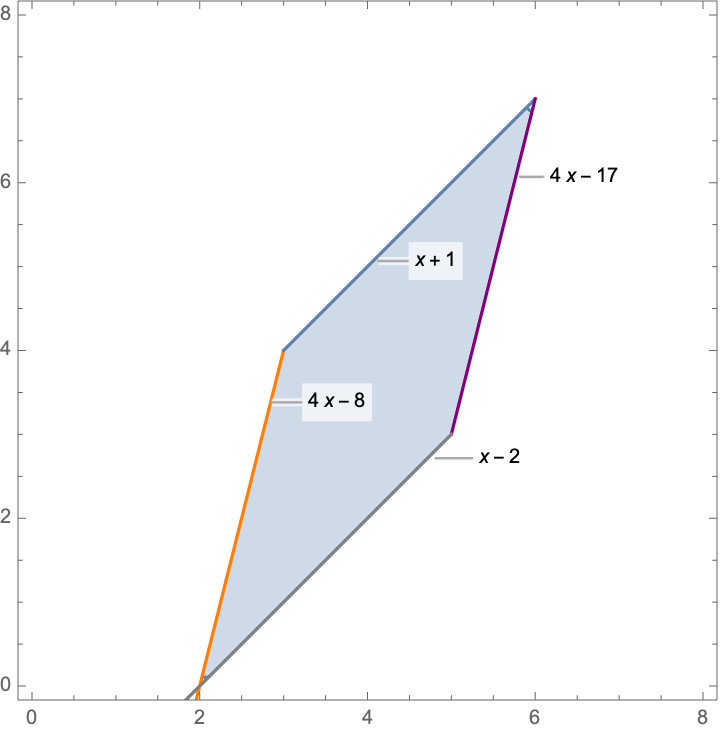
\includegraphics[width = 0.7\linewidth]{Figure/2.1.png}
\end{figure}

\par Please calculate the weight of this window for him, namely 
\begin{equation*}
    \iint_R 6x-3y \,dA.
\end{equation*}
where $R$ describes the region of the window. Notice that you may want to use the following transformation:
\begin{equation*}
    x = \frac{1}{3}(v - u), \quad y = \frac{1}{3}(4v - u).
\end{equation*}

%-Part 2.2--------------------------------------------------------------------------------------------------------
\subsection*{2.2 Breathe! (4 Marks)}
\par After some struggles, Pingping and Bangbang finally get into the building. When they see the machine, they are 
shocked by how complicated it is. It has too many switches on it! Pingping is too excited about it, so he decides to just lie in the machine and closed it. 

\par After 5 minutes, Pingping feels a little bit hypoxia(loosing air to breathe); meanwhile, Bangbang is reading the 
instruction of this machine, he find out that when one wants to use it, he(she) needs to turn on the air 
circulation! Bangbang bet that Pingping does not do this, which is true. But Bangbang is not able to open the machine
from the outside, in this emergency situation, Bangbang decides to call the security for help...

\par What is Pingping doing then? He finds out that the whole shape of the machine can be described as 
\begin{equation*}
    x = 2y^2 + 2z^2 - 5 
\end{equation*}
with a cap described by 
\begin{equation*}
    x = 1.
\end{equation*}
 
\par Furthermore, it seems to him that the current oxygen density is given by the equation 
\begin{equation*}
    d(x,y,z) = yz. 
\end{equation*}

\par Disregards how Pingping comes up with all of these, please find the total amount of oxygen left in the 
machine for him! Namely, please calculate 
\begin{equation*}
    \iiint_M yz\,dV
\end{equation*}
where $M$ is the region of the machine described above. 

\par Wait, what? You want me to provide you the graph of $M$ just like the last question? Hey, it's time to grow 
up! \\
\hfill (p.s. Don't always trust Pingping's intuition, he may be wrong at some time!)


%-Part 2.3--------------------------------------------------------------------------------------------------------
\subsection*{2.3 FIVE Dimension (3 Marks)}
\par After Pingping konws that his intuition is wrong, he feels sad. He opens the machine and climbs out of it. But 
he does not see Bangbang. The only thing he sees is the instruction book for this virtual machine, which is left 
on the floor opening to the page that explains how to turn on the air circulation function for this machine. 

\par Pingping is excited again! He immediately decides to go back to the virtual machine, turn on the air 
circulation function and start to explore the magic of this machine. After some time, when Pingping finally 
finds out how to enter the virtual reality, Bangbang and the security arrive. The security is so afraid to be 
fired becasue of his inattention, so he decides to open the machine from the outside by force. But at that time,
the system of the machine detects this and decides to turn on its protection mechanism. 

\par Just then, Pingping starts to see a strange shape that he never saw before. He is fascinated by it. It's so 
complex, so beautiful, and so symmetric. Long time passes bt and Pingping murmurs: "It's a five dimensional ball... I 
know it... It must be... It is a five dimensional sphere with radius $R$..."

\par He decide to calculate the volume of this five dimensional ball, can you help him? Namely, please calculate 
\begin{equation*}
    \abs{B_5} = \idotsint_{B^5}1 \,dB^5. 
\end{equation*}

\par What? again? You want me to provide you a graph for that ball? Get out of here!\\
\hfill (p.s. Maybe you will need the result from \textbf{1.3}, but who knows...)

%-Part 2.4--------------------------------------------------------------------------------------------------------
\subsection*{2.4 Challenge from Bangbang (4 Marks)}
\par After solving the volume of a five dimensional ball, the whole virtual reality world darks out. And then, 
Pingping is forced to quit from the virtual reality to reality. He notices that there is a warning from the machine 
telling him that someone is trying to breakout the machine from outside. 

\par Pingping thinks that it is because Bangbang is too jealous that he is not the first one to try this machine, so he
yells out: "How can you cut down the power and do this to me? I'm enjoying the magic of this machine! I even 
saw a five dimensional ball!"

\par Bangbang:"Stop saying that nonsense anymore! If you are able to identify a five dimensional ball, you must be able to
solve this! I bet you can't!"

\par As soon as Bangbang challenges Pingping, Pingping opens the machine and jumps out. He is never \textbf{insulted} like 
this before! No one can judge his ability of doing integration! He yells at Bangbang: "Show me what you get!" 
Bangbang slowly speaks out the integration, which is
\begin{equation*}
    \int_\R \frac{\cos (x)}{x^2+1}\,dx. 
\end{equation*}

\par After Bangbang is done, Pingping sneers at him. "Ha... Haha... Hahaha... Are you kidding me? Only one variable? 
You are insulting me again! I'll do this in 2 minutes!"

\par Please help Pingping to find out the answer of this integral!\\

\hfill (Probably not solving it in 2 minutes is also OK, but Pingping will be upset...)
\newpage
%-Part 3 ---------------------------------------------------------------------------------------------------------
\section*{Part 3 : Things May Not Act as What You Thought}

Suzumiya Haruhi is Watahashi Yasumi's math tutor. She is teaching her how to solve integral problems. She does not like ordinary approach and too normal daily life. She looks forward to making the world more interesting and to spreading cheer and excitement. Some problems may seem simple, but indeed they are tricky. Some problems seems huge and complicated, but they are easy to solve. Some problems have the most ugly parameters, but the solution is quite concise. These are quite interesting problems in Haruhi's mind. Haruhi offered Yasumi three integral exercises. Suppose you are Yasumi, please solve these problems.
\par In your answer, leave $\arctan$ as what they are. Do not calculate them out except that you can let $\arctan 0 = 0$. Do not leave any square root in the denominator. Do not write $\log$ and $\arctan$ more than once in your answer.

%-Part 3.1--------------------------------------------------------------------------------------------------------
\subsection*{3.1 Simple Integral (3 Marks)}
\begin{equation*}
    K = \int^{\sqrt{2}}_{1} \frac{1}{1 + x^4}\,dx. 
\end{equation*}

%-Part 3.2--------------------------------------------------------------------------------------------------------
\subsection*{3.2 Complicated Double Integral (3 Marks)}
\begin{equation*}
    M=\iint_{x^{2}+y^{2} \leqslant 1}\left|\frac{x+y}{\sqrt{2}}-x^{2}-y^{2}\right| \mathrm{d} x \mathrm{~d} y.
\end{equation*}

%-Part 3.3--------------------------------------------------------------------------------------------------------
\subsection*{3.3 Ugly Line with a Beautiful Line Integral Result (2 Marks)}
Given the curve $\Gamma$
\begin{equation*}
    \left\{\begin{array}{l}
(x-y)^{2}=a(x+y) \\
x^{2}-y^{2}=\frac{9}{8} z^{2}. 
\end{array}\right.
\end{equation*}
calculate the length $I$ on $\Gamma$ from $A:\left(0, 0, 0\right)$ to $B:\left(1, y_0, z_0\right)$. 

%-Part 3.4--------------------------------------------------------------------------------------------------------
\subsection*{3.4 Last Exercise for Yasumi (4 Marks)}
\par Yasumi successfully solved the three questions in \textbf{Part 3} and it's time to go to SOS Brigade to have some fun in after-class club activities. In the club activity room, Haruhi is quite proud that Yasumi's ability to solve integral has improved a lot. Now she asks Yasumi to solve one problem on the blackboard. Suppose you are Yasumi, please solve this problem.

\begin{equation*}
    P=\iiint_{\Omega}\left[\frac{1}{y z} \frac{\partial F}{\partial x}+\frac{1}{x z} \frac{\partial F}{\partial y}+\frac{1}{x y} \frac{\partial F}{\partial x}\right] \mathrm{d} x \mathrm{~d} y \mathrm{~d} z. 
\end{equation*}
where $\omega=1 \leqslant y z \leqslant 2,1 \leqslant x z \leqslant 2,1 \leqslant x y \leqslant 2$ and $F=2 x + M y + \lfloor I \rfloor z$. 

\begin{flushright}
    Based on characters in \textsl{The Surprise of Haruhi Suzumiya}, Nagaru Tanigawa
\end{flushright}

\newpage
%-Part 4 ---------------------------------------------------------------------------------------------------------
\section*{Part 4 : }
\par AppleDog and DT, both are robot players, would like to create and run a small video website in their spare time. To achieve this, they need to define a system for their website that assigns ranks for existing videos and videos under review. By investigating the ranking system of \textsl{Piggy Piggy} (a famous video website), they list some criteria for their system.
\begin{itemize}
    \item[(a)] The score of a video decreases as time (\emph{$x_1$}) passes by;
    \item[(b)] The score of a video increases as the heat (\emph{$x_2$}) of the topic of the video increases;
    \item[(c)] The score of a video increases as the number of views (\emph{$x_3$}) of it increases;
    \item[(d)] The score of a video increases as the total number of likes and collections (\emph{$x_4$}) it obtains increases;
    \item[(e)] $x_2$, $x_3$, $x_4$ are all related to time \emph{$x_1$}. 
\end{itemize}
\par After some thought, DT derives a function 
\begin{equation*}
    f:\R^4 \to \R,\quad f(x_1, x_2, x_3, x_4) = 2 x_2(\alpha + x_1^2)^{-1} + x_4e^{x_4}(1 + x_3)
\end{equation*}
where $x_i$'s are defined as above, and $\alpha > 0$ is a parameter depending on the type of a video. The score of an \textsl{existing video} is the line integral of $f$ along its data curve
\begin{equation*}
    \gamma(t)=(t,x_2(t),x_3(t),x_4(t)), 
\end{equation*}
and the predicted score of a video \textsl{under review} is the integral of $f$ over the domain $E$ bounded by
\begin{equation*}
    \begin{split}
        0 \leq x_1\leq 7;& \quad 0 \leq x_2 \leq \sqrt{(\beta + x_1^2)^{-1}};\\
        0 \leq x_3 \leq 3;& \quad 0 \leq x_4 \leq \log(1 + x_3),\\ 
    \end{split}
\end{equation*}
where $\beta > 0$ is a parameter depending on the topic of a video, and "$\log$" is the inverse function of $e^x$.
\par AppleDog is curious about DT's model, so she tries with some examples. \textbf{Your task is to help Appledog calculate the results}. 

%-Part 4.1--------------------------------------------------------------------------------------------------------
\subsection*{4.1 Score of Existing Video (2 Marks)} 
\par Suppose in the first 7 days the data of a video (i.e., heat, number of views, etc.) follows the curve $\mathcal{C}$ parametrized by 
\begin{equation*}
    \gamma:[0,7]\to \R^4,\quad \gamma(t) = (t, \sqrt{\alpha}, t, 0)
\end{equation*}

\par Determine the score of this video, i.e., evaluate the integral below (\textbf{express your answer in $\alpha$ and $\beta$}) 
\begin{equation*}
    \int_{\mathcal{C}}f. 
\end{equation*}

\par Then determine the value of $\alpha$ when the score of this video is $2\sqrt{2}$. This \emph{$\alpha$} will be used in \textbf{4.4}. 

%-Part 4.2--------------------------------------------------------------------------------------------------------
\subsection*{4.2 Area of Domain $E$ (3 Marks)} 
AppleDog first wants to see the area of $E$, where $E$ is defined above. Help her calculate it (\textbf{express your answer in $\alpha$}).  

%-Part 4.3--------------------------------------------------------------------------------------------------------
\subsection*{4.3 Predicted Score of Video Under Review (4 Marks)}
Help AppleDog calculate the predicted score of a video under review, i.e., evaluate the following integral, where $f$ is defined as above (\textbf{express your answer in $\alpha$ and $\beta$}) 
\begin{equation*}
	    \int_0^7 \int_0^{\sqrt{(\beta + x_1^2)^{-1}}} \int_0^{3} \int_0^{\log(1 + x_3)} f(x_1, x_2, x_3, x_4)\,dx_4 dx_3 dx_2 dx_1.
\end{equation*}

%-Part 4.4--------------------------------------------------------------------------------------------------------
\subsection*{4.4 Challenge From AppleDog (3 Marks)}
\par Knowing that DT has been attending robot competitions since 16, AppleDog believes that he must be smart and good at math. Thus, she gives him an integration as a reward for his contribution to the video ranking system: 
\par Let \emph{$\alpha$} be the value calculated in \textbf{4.1}. Suppose that $f:[0,1] \to \mathbb{R}$ is continuous and 
\begin{equation*}
    \int_0^1 f(x) dx = \alpha. 
\end{equation*}
Evaluate the following integral (your answer \textbf{should not} contain \emph{$\alpha$}). 
\begin{equation*}
    \int_0^1 \int_0^x \int_0^y f(x)f(y)f(z)\,dzdydx. 
\end{equation*} 
~\\ 

\begin{flushright}
    The story is based on the TV series "DT/AppleDog's Time", 2021
\end{flushright}


\newpage
%-Answer----------------------------------------------------------------------------------------------------------
\section*{Answer}
%-Part 1 ---------------------------------------------------------------------------------------------------------

\par \textbf{Answer for 1.1: }
\begin{equation*}
    \frac{\ln^2(x)}{2} + \frac{1}{2}
\end{equation*}

\par \textbf{Answer for 1.2: }
\begin{equation*}
    \sin(a)
\end{equation*}

\par \textbf{Answer for 1.3: }
\begin{equation*}
    \frac{4}{3}
\end{equation*}

%-Part 2 ---------------------------------------------------------------------------------------------------------
\par \textbf{Answer for 2.1: }
\begin{equation*}
    \frac{243}{2}
\end{equation*}

\par \textbf{Answer for 2.2: }
\begin{equation*}
    0
\end{equation*}

\par \textbf{Answer for 2.3: }
\begin{equation*}
    \frac{8\pi^2}{15}R^5
\end{equation*}

\par \textbf{Answer for 2.4: }
\begin{equation*}
    \frac{\pi}{e}
\end{equation*}

%-Part 3 ---------------------------------------------------------------------------------------------------------

\par \textbf{Answer for 3.1: }
\begin{equation*}
    -\frac{\sqrt{2}}{8}\ln \frac{3+2\sqrt{2}}{5}+\frac{\sqrt{2}}{4}\arctan \frac{1}{2}
\end{equation*}

\par \textbf{Answer for 3.2: }
\begin{equation*}
    \frac{9\pi}{16}
\end{equation*}

\par \textbf{Answer for 3.3: }
\begin{equation*}
    \sqrt{2}
\end{equation*}

\par \textbf{Answer for 3.4: }
\begin{equation*}
    \left(1+\frac{9\pi}{16}\right)\ln^2 2 + 2\ln 2
\end{equation*}

%-Part 4 ---------------------------------------------------------------------------------------------------------

\par \textbf{Answer for 4.1: }
\begin{equation*}
        2\sqrt{2}\arctan(7/\sqrt{\alpha}), \quad \alpha = 28^2/\pi^2\ \text{or}\ \alpha = 784/\pi^2
\end{equation*}

\par \textbf{Answer for 4.2: }
\begin{equation*}
    \begin{split}
        &(4 \log 4 - 3)\arcsinh (\frac{7}{\sqrt{\beta}})\quad \text{or}\\
        &(4 \log 4 - 3)\log (\frac{\sqrt{49+\beta} + 7}{\sqrt{\beta}})\quad \text{or}\\
        &(4 \log 4 - 3)\log(\sqrt{(\frac{7}{\sqrt{\beta}})^2+1} + \frac{7}{\sqrt{\beta}})
    \end{split}
\end{equation*}

\par \textbf{Answer for 4.3: }
\begin{equation*}
    \frac{4\log 4 - 3}{\beta - \alpha}\left[\frac{\arctan(7/\sqrt{\alpha})}{\sqrt{\alpha}} - \frac{\arctan(7/\sqrt{\beta})}{\sqrt{\beta}}\right] 
    + (\frac{64}{3}\log 4 - \frac{41}{2})\arcsinh(\frac{7}{\sqrt{\beta}})
\end{equation*}

\par \textbf{Answer for 4.4: }
\begin{equation*}
    \frac{392}{3\pi^2} \quad \text{or} \quad \frac{28^2}{6\pi^2} \quad \text{or}\quad \frac{784}{6\pi^2}
\end{equation*}


\end{document}
